\documentclass{standalone}
\usepackage{tikz}
\usepackage{ctex,siunitx}
\usepackage{tkz-euclide}
\usepackage{amsmath}
\usetikzlibrary{patterns, calc}
\usetikzlibrary {decorations.pathmorphing, decorations.pathreplacing, decorations.shapes,}
\begin{document}
\small
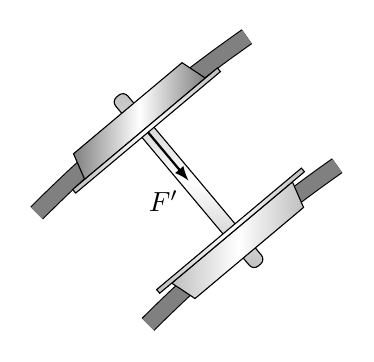
\begin{tikzpicture}[>=latex,scale=1]
  % \useasboundingbox(,)rectangle(,);
  \draw[double=gray,double distance=2mm](135:20)arc(135:125:20);
  \draw[double=gray,double distance=2mm](135:18)arc(135:125:18);
  \begin{scope}[shift=(130:19),rotate=-50]
    \fill[top color=lightgray,bottom color=lightgray,middle color=white,rounded corners=0.8mm,draw=black](-1.4,0.1)rectangle(1.4,-0.1);
    \fill[left color=gray,right color=gray,middle color=white,draw=black]
    (-1.2,-0.9)--(-1.2,0.9)--(-0.86,1)--(-0.86,-1)--cycle;
    \fill[left color=lightgray,right color=lightgray,middle color=white,draw=black]
    (-0.8,-1.2)rectangle(-0.86,1.2);
    \fill[left color=lightgray,right color=lightgray,middle color=white,draw=black]
    (1.2,-0.9)--(1.2,0.9)--(0.86,1)--(0.86,-1)--cycle;
    \fill[left color=lightgray,right color=lightgray,middle color=white,draw=black]
    (0.8,-1.2)rectangle(0.86,1.2);
    \draw[thick,->](-0.8,0)--++(0.8,0)node[below left]{$F'$};
  \end{scope}
\end{tikzpicture}
\end{document}